\documentclass[12pt]{beamer}
\usepackage[T1]{fontenc}
\usepackage[utf8]{inputenc}
\usepackage{lmodern}
\usepackage[english]{babel}
\usepackage{xcolor}
\usepackage{pgf,tikz}
%\usetikzlibrary{calc}
\usepackage{amssymb,amsmath,array,bm}
\usepackage[T1]{fontenc}
\usepackage[utf8]{inputenc}
\usepackage{hyperref}
\usepackage{multicol}
\usepackage{tabularx}


\def\fnmark#1{{\small}$^#1$}
\def\fnote#1#2{$^#1\;$\texttt{#2}\\}

\usepackage{verbatim}
%\usepackage[active,tightpage]{preview}
\usetheme{Madrid}

\usetikzlibrary{positioning,shapes,shadows,arrows}
\tikzstyle{myarrow}=[<-, >=open triangle 90, thick]
\tikzstyle{line}=[-, thick]

\begin{document}
	
	\date[SRS'17]{Summer Research School \\ 2017}
	\institute[SHSM]{Sofia High School of Mathematics \\ Sofia, Bulgaria}
	\author[Mr. Zlatogor Minchev, Alex]{
		\begin{table}[]
			\begin{tabular}{rl}
				\normalsize{Author:\      } & \normalsize{Alex Ivanov Tsvetanov} \\
				\scriptsize{Mentors:     } & \scriptsize{Assoc. Prof. Zlatogor Minchev} \\
				& \scriptsize{Assist. Prof. Emil Kelevedzhiev} \\
			\end{tabular}
		\end{table}
	}
	\title[ArtTeach]{Artificial teacher}
	
	\begin{frame}
		\titlepage
	\end{frame}

	\begin{frame}
		\frametitle{Introduction}
		\begin{block}{}
			The core aim of our project is to create system that combines these techniques and to build "artificial teacher" that combines best practices in organizing training so that it will be interesting, useful and much easier for the students. The most important part of our project is to fertilize students, showing them that their subjects is not as difficult as sound
		\end{block}
	\end{frame}
	
	\begin{frame}
		\frametitle{Why it is useful?}
		\begin{block}{It's useful ...}
			\begin{itemize}
				\item for self-study
				\item for modernizing education
			\end{itemize}
		\end{block}
		\begin{block}{It allows young people ...}
			\begin{itemize}
				\item to touch new technologies
			\end{itemize}
		\end{block}
		\begin{block}{It can ...}
			\begin{itemize}
				\item provoke the interest of young people in the subjects
			\end{itemize}
		\end{block}
	\end{frame}
	\begin{frame}
		\frametitle{Architecture}
		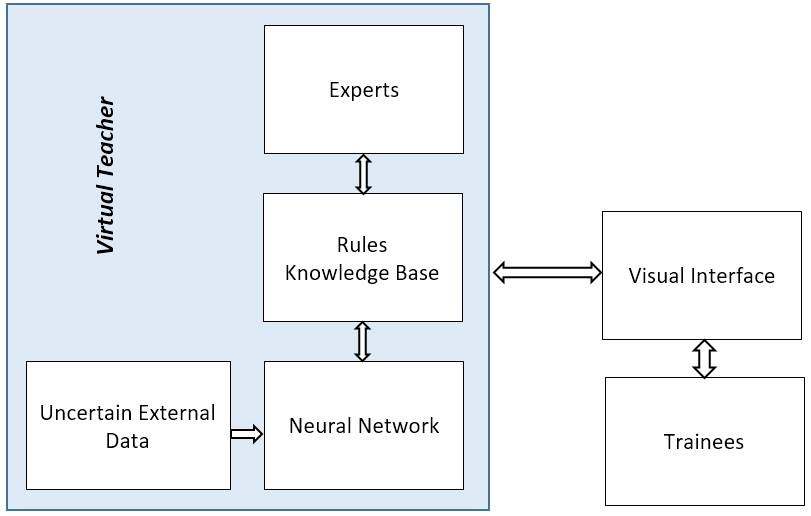
\includegraphics[width=\textwidth]{.../schema.jpg}
	\end{frame}
	\begin{frame}
		\frametitle{Innovations?}
		\begin{itemize}
			\item It combines 2 new technologies - Machine learning/Artificial intelligence/Neural Network \& Virtual Reality
			\item Learning is closer to the new generations
			\item Learning is more interactive
		\end{itemize}
	\end{frame}
	\begin{frame}
		\frametitle{What is ready?}
		\begin{itemize}
			\item Neural network API based on statistics
			\item Prototype of user interface
		\end{itemize}
	\end{frame}
	\begin{frame}
		\frametitle{What is next?}
		\begin{itemize}
			\item Improvement of API (it will start to use "expert system") 
			\item Finishing 3D human model
			\item Building library for voice/text communication with students
			\item Finishing web-based user interface
			\item Building API-based mobile application
			\item Building VR application
		\end{itemize}
	\end{frame}
	\begin{frame}
		\begin{center}
			{\Huge Live prototype demo} \\ \vspace{1cm}
			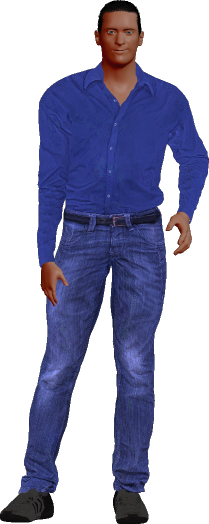
\includegraphics[scale=0.25]{../bad_boy.png}
		\end{center}
	\end{frame}
	\begin{frame}
		Special thanks for:
		\begin{itemize}
			\item \href{https://bg.linkedin.com/in/zlatogor-minchev-a101b85}{Assoc. Prof. Zlatogor Minchev} \\
			\item \href{https://bg.linkedin.com/in/emil-kelevedjiev-34727310b}{Assist. Prof. Emil Kelevedjiev} \\\par
		\end{itemize}
		\vspace{0.5cm}
		Acknowledges for:
		\begin{itemize}
			\item \href{http://www.math.bas.bg/omi/hssimi/}{High School Students Institute of Mathematics and Informatics}
			\item \href{http://www.math.bas.bg/}{Bulgarian Academy of Sciences}
			\item \href{http://www.smg.bg}{Sofia High School of Mathematics}
			\item \href{https://www.vrexpress.bg/}{VR Express}
		\end{itemize}
	\end{frame}
	
	\begin{frame}
	\frametitle{Resources}
		\begin{itemize}
			\item
			{\itshape Artificial Intelligence: A Modern Approach, \\ 3rd Edition, Prentice Hall, 2010}. \\
			\texttt{Stuart Russell \& Peter Norvig.} \\
			\item
			{\itshape Virtual\ objects\ seem\ totally\ real}.
			\\
			\item
			{\itshape Amelia}.
			\texttt{http://www.ipsoft.com/amelia/}. \\
			\item
			{\itshape The Future Of Chatbots And Artificial Intelligence}.
			\item
			{\itshape Your DNA Avatar - What Happens When Artificial Intelligence Meets Cutting-Edge Genetics?}.
			\item%{gcc}
			{\itshape GNU Compiler Collection}.
			\texttt{https://gcc.gnu.org/}. \\
			Copyright \copyright\  2009 Free Software Foundation, Inc.
			\item%{mariadb}
			{\itshape MariaDB}.
			\texttt{https://mariadb.org/}. \\
			Copyright \copyright\  2017 MariaDB Foundation
			\item%{mariadb}
			{\itshape MariaDB++}.
			\texttt{https://mariadb.org/}. \\
			Copyright \copyright\  2017 MariaDB Foundation
			\item%{latex}
			{\itshape \LaTeX}.
			\texttt{https://www.latex-project.org/}.
		\end{itemize}
	\end{frame}
	
	\begin{frame}
	\begin{center}
	{\Huge Questions}\\
	
\includegraphics[scale=0.25]{../questions.png}
	\end{center}
	\end{frame}
	
	\begin{frame}
	\begin{center}
	{\Huge Thank you\\for\\the attention!}
	\end{center}
	\end{frame}

\end{document}
